% 由 tutorial.tex 自动拆分为第 14 章
\chapter{torch 实现与训练对比}
\section{等价结构}

\begin{lstlisting}[caption={tinytf\_torch.py 的核心（与 numpy 版一一对应）}]
class Block(nn.Module):
    def forward(self, z, mask):
        B, T, d = z.shape
        q, k, v = self.qkv(self.ln1(z)).chunk(3, dim=-1)
        q, k, v = [t.view(B, T, self.h, self.nh).transpose(1, 2) for t in (q, k, v)]
        s = (q @ k.transpose(-1, -2)) / math.sqrt(self.nh)
        a = torch.softmax(s.masked_fill(mask, -1e9), dim=-1)
        z = z + self.proj((a @ v).transpose(1, 2).reshape(B, T, d))
        return z + self.fc2(F.gelu(self.fc1(self.ln2(z))))
\end{lstlisting}

两版共享权重布局：\texttt{state\_from\_numpy()} 把 numpy 的字典映射成 \texttt{state\_dict}，
反向映射是 \texttt{numpy\_from\_state()}。这让我们可以做三件事：
验证梯度、以 numpy 做推理、以及把生产权重装进 numpy 做可视化。

\section{训练对比}

同初始化、同数据（52,164 个训练窗口）、同批次顺序、同学习率调度，各训 8 个 epoch：

\begin{center}
\small
\begin{tabular}{@{}lccc@{}}
\toprule
 & 训练损失（8 epoch 末） & 验证损失 & 耗时 \\
\midrule
numpy（手写反向） & $3.60\times10^{-3}$ & $3.694\times10^{-3}$ & $142$\,s \\
torch（autograd） & $3.60\times10^{-3}$ & $3.695\times10^{-3}$ & $35$\,s \\
\midrule
差异 & $1.7\times10^{-7}$ & $1.3\times10^{-7}$ & 加速 $4.1\times$ \\
\bottomrule
\end{tabular}
\end{center}

\begin{figure}[htbp]
\centering
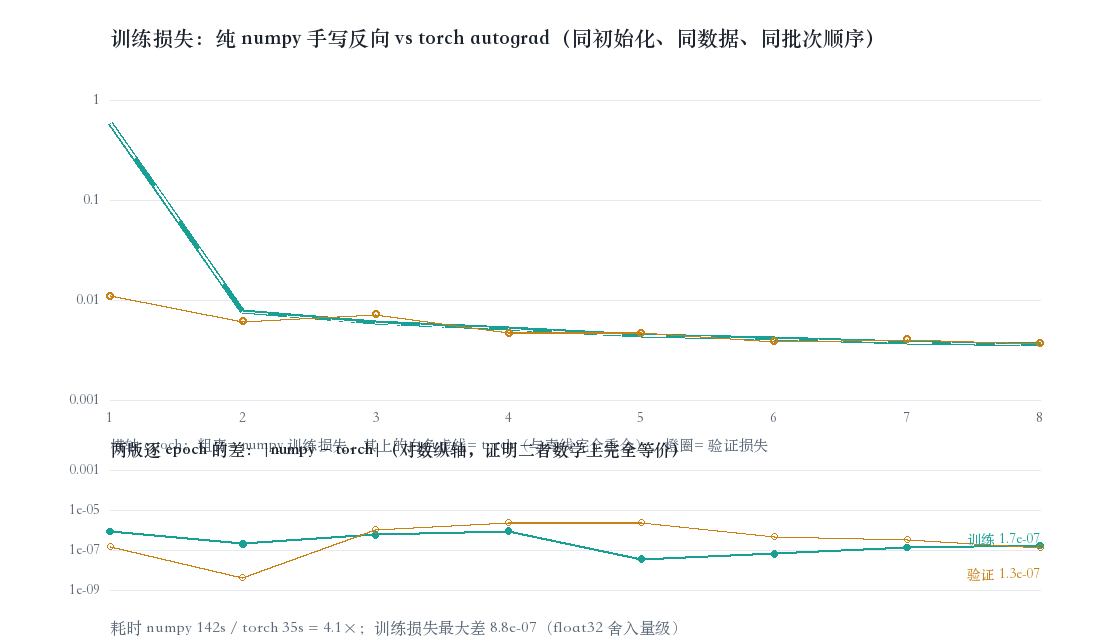
\includegraphics[width=0.96\linewidth]{fig_loss.png}
\caption{上：训练/验证损失；粗青线是 numpy，其上白色虚线是 torch（两者完全重合）。
下：两版逐 epoch 的绝对差，稳定在 float32 舍入量级 $10^{-7}$。}
\end{figure}

